

\documentclass[conference]{IEEEtran}
\IEEEoverridecommandlockouts
% The preceding line is only needed to identify funding in the first footnote. If that is unneeded, please comment it out.
\usepackage{cite}
\usepackage{amsmath,amssymb,amsfonts}
\usepackage{algorithmic}
\usepackage{graphicx}
\usepackage{textcomp}
\usepackage{xcolor}
\def\BibTeX{{\rm B\kern-.05em{\sc i\kern-.025em b}\kern-.08em
    T\kern-.1667em\lower.7ex\hbox{E}\kern-.125emX}}

%\documentclass[11pt]{article} 
%\usepackage{times}

%\usepackage{pifont}
%\usepackage{bm}
%\usepackage{epsfig}
%\usepackage{psfig}
%\usepackage{tabularx}
%\usepackage{amssymb}
%\usepackage{latexsym}
%\usepackage{amsmath}
%\usepackage{delarray}
%\usepackage{moreverb}
%\usepackage{xspace}
%\usepackage{algorithm}
%\usepackage{algorithmic}

%\usepackage{lscape}
%\usepackage{changebar}
%\usepackage{graphicx}
%\usepackage{graphics}
%\usepackage{mflogo}
%\usepackage{xspace}
%\usepackage{texnames}
%\usepackage{rotating}
%\usepackage{alltt}

%\usepackage{amsmath}
%\usepackage{epsfig}
%\usepackage{booktabs,paralist}

\def\firmopsa{d}
\def\firmopsb{d}
\newcommand\AssignTags{TagIt}


% Definitions
% -----------
\def\x{{\mathbf x}}
\def\L{{\cal L}}
\def\spiral{SPIRAL\xspace}

\newcommand{\pred}{{}}

\newcommand{\tensor}[0]{\otimes}
\newcommand{\inv}[1]{{1{/}{#1}}}
%\newcommand{\inv}[1]{$\textstyle\frac{1}{#1}$}
\newcommand{\DFT}{\operatorname{\bf DFT}}
\newcommand{\WHT}{\operatorname{\bf WHT}}
\newcommand{\FIR}{\operatorname{\bf FIR}}
\newcommand{\one}[0]{{I}}
\newcommand{\eq}[0]{{=}}
\newcommand{\Tensor}[2]{#1{\tensor}#2}
\newcommand{\TensorT}[3]{{#1{\tensor}#2}_{#3}}
\newcommand{\SPw}[2]{{\prec}#1,#2{\succ}}
\newcommand{\SPr}[2]{{<}#1,#2{>}}

\newcommand{\WTensorI}[2]{\Tensor{\WHT_{#1}}{\one_{#2}}}
\newcommand{\ITensorW}[2]{\Tensor{\one_{#1}}{\WHT_{#2}}}
\newcommand{\Wht}[2]{(\WTensorI{\WHT_{#1}}{#2})(\ITensorW{#1}{#2})}

\newcommand{\Times}[2]{{#1}{\times}{#2}}
\newcommand{\EQ}{{=}}
\newcommand{\Space}{{ S}}
\newcommand{\PEQ}{{{+}{=}}}
\newcommand{\SEQ}{{{-}{=}}}
\newcommand{\h}{\psi}
\newcommand{\balpha}{\bm{\alpha}}
\newcommand{\bgamma}{\bm{\gamma}}
\newcommand{\bbeta}{\bm{\beta}}
\newcommand{\bmu}{\bm{\mu}}
\newcommand{\bsigma}{\bm{\sigma}}


\newcommand{\f}{\varphi}
\newcommand{\Z}{\mathbb{Z}}
\newcommand{\A}{\mathbb{A}}
\newcommand{\B}{{\bf B}}
\newcommand{\X}{\mathbb{X}}
\newcommand{\T}{\mathbb{T}}
%\newcommand{\Q}{\mathbb{Q}}
\newcommand{\N}{\mathbb{N}}
\newcommand{\R}{\mathbb{R}}
\newcommand{\CC}{{\Gamma}}
\newcommand{\D}{\mathbb{D}}
\newcommand{\M}{\mathbb{M}}
\newcommand{\F}{\mathbb{F}}
\newcommand{\ST}{\mathbb{S}}
\newcommand{\Vc}[1]{{\boldsymbol #1}}
\newcommand{\fl}[1]{{\lfloor {#1} \rfloor}}
\newcommand{\cl}[1]{{\lceil {#1} \rceil}}
\newcommand{\half}[1]{{\frac{#1}{2}}}
\newcommand{\q}[1]{\Times{\cl{#1}}{\cl{#1}}}
\newcommand{\qq}[1]{\Times{\cl{#1}}{\fl{#1}}}
\newcommand{\qqq}[1]{\Times{\fl{#1}}{\cl{#1}}}
\newcommand{\qqqq}[1]{\Times{\fl{#1}}{\fl{#1}}}
\newcommand{\size}[1]{\sigma(#1)}
\newcommand{\Size}[3]{\sigma(\Vc{#1})\EQ\Times{#2}{#3}}
\newcommand{\n}{(\frac{n}{2})}
\newcommand{\m}{(\frac{n-1}{2})}
\newcommand{\Ceil}[1]{{\cl{\half{#1}}}}
\newcommand{\Floor}[1]{{\fl{\half{#1}}}}

\newcommand{\Endash}{{--}}
\newcommand{\Emdashbegin}{{---}}
\newcommand{\Emdashend}{{---}~}

\newcommand{\Transducer}[1] {{\mathbf #1 }}
\newcommand{\Triangle}[1] {{\vartriangle\!\! #1 }}


\newcommand{\AO}  {\Times{\Ceil{m}}{\Ceil{n}}}
\newcommand{\AI} {\Times{\Ceil{m}}{\Floor{n}}}
\newcommand{\AII}{\Times{\Floor{m}}{\Ceil{n}}}
\newcommand{\AIII} {\Times{\Floor{m}}{\Floor{n}}}
\newcommand{\BO}  {\Times{\Ceil{n}}{\Ceil{p}}}
\newcommand{\BI} {\Times{\Ceil{n}}{\Floor{p}}}
\newcommand{\BII}{\Times{\Floor{n}}{\Ceil{p}}}
\newcommand{\BIII} {\Times{\Floor{n}}{\Floor{p}}}
\newcommand{\CO}  {\Times{\Ceil{m}}{\Ceil{p}}}
\newcommand{\CI} {\Times{\Ceil{m}}{\Floor{p}}}
\newcommand{\CII}{\Times{\Floor{m}}{\Ceil{p}}}
\newcommand{\CIII} {\Times{\Floor{m}}{\Floor{p}}}

\newcommand{\I}[2]{\Times{\Ceil{#1}}{\Ceil{#2}}}
\newcommand{\II}[2]{\Times{\Ceil{#1}}{\Floor{#2}}}
\newcommand{\III}[2]{\Times{\Floor{#1}}{\Ceil{#2}}}
\newcommand{\IV}[2]{\Times{\Floor{#1}}{\Floor{#2}}}


\newcommand{\Q}[2]{\Vc{#1}_{#2}}

\newcommand{\QAO}{{\Vc{A}_{0}}}
\newcommand{\QAI}{\Vc{A}_{1}}
\newcommand{\QAII}{\Vc{A}_{2}}
\newcommand{\QAIII} {\Vc{A}_{3}}

\newcommand{\QBO}  {\Vc{B}_{0}}
\newcommand{\QBI} {\Vc{B}_{1}}
\newcommand{\QBII}{\Vc{B}_{2}}
\newcommand{\QBIII} {\Vc{B}_{3}}

\newcommand{\QCO}  {\Vc{C}_{0}}
\newcommand{\QCI} {\Vc{C}_{1}}
\newcommand{\QCII}{\Vc{C}_{2}}
\newcommand{\QCIII} {\Vc{C}_{3}}
\newcommand{\FIGsize}[2]{{width={#1}, height={#2}}}

\newcommand{\Mod}[2]{{#1}{\text{ \bf mod }}{#2}}

\newcommand{\TableRef}[1]{Table \ref{#1}}
\newcommand{\FigureRef}[1]{Figure \ref{#1}}
\newcommand{\SectionRef}[1]{Section \ref{#1}}
\newcommand{\EquationRef}[1]{Equation \ref{#1}}
\newcommand{\OnPageRef}[1]{on page \pageref{#1}}

% Formatting
% ----------
%\setlength{\evensidemargin}{0mm}
%\setlength{\oddsidemargin}{0mm}
%\setlength{\textwidth}{6.5in}
%\setlength{\textheight}{9.5in}
%\setlength{\topmargin}{0in}
%\setlength{\headheight}{0in}
%\setlength{\headsep}{0mm}

\newenvironment{noinds_itemize}{\begin{list}{$\bullet$}
{\setlength{\rightmargin}{0em}
\setlength{\leftmargin}{1.2em}
\setlength{\itemsep}{0em}
\setlength{\topsep}{0em}
\setlength{\parsep}{0em}}}{\end{list}}



\newcommand{\mypar}[1]{{\bf #1.}}
\newcommand{\mytag}[2]{[#1]_{#2}}
\sloppy

%% jan 01, 2009 - dasdan - removed 'final' pdflatex cannot work with it.
%\usepackage[final=true,bookmarks=true,bookmarkstype=toc,colorlinks=true, linkcolor=blue,citecolor=blue]{hyperref}
%\usepackage[bookmarks=true,bookmarkstype=toc,colorlinks=true, linkcolor=blue,citecolor=blue]{hyperref}

% width fraction, mflops, relative, caption, label
\newcommand{\doublefigure}[5]{{\begin{figure}%
\centering %
\includegraphics[width=#1\linewidth]{#2}
\includegraphics[width=#1\linewidth]{#3}%\figurebox{#1\linewidth}{}{}[#2]
%\figurebox[#1\linewidth]{}{}[#3] %
\caption{#4}%bio                 
\label{#5}%
\end{figure}}}

\newcommand{\Doublefigure}[5]{{\begin{figure*} %
\centering %
%\includegraphics[height=#1\linewidth,angle=-90]{#2}%
%\includegraphics[height=#1\linewidth,angle=-90]{#3} %
\includegraphics[width=#1\linewidth]{#2} \\  %
\includegraphics[width=#1\linewidth]{#3}%
%\figurebox{#1\linewidth}{}{}[#2]
%\figurebox{#1\linewidth}[#3] %
\caption{#4}%
\label{#5}%
\end{figure*}}}

\newcommand{\DDoublefigure}[5]{{\begin{figure*} %
\centering %
%\includegraphics[height=#1\linewidth,angle=-90]{#2}%
%\includegraphics[height=#1\linewidth,angle=-90]{#3} %
\includegraphics[width=#1\linewidth, angle=90]{#2}   %
\includegraphics[width=#1\linewidth, angle=90]{#3}%
%\figurebox{#1\linewidth}{}{}[#2]
%\figurebox{#1\linewidth}[#3] %
\caption{#4}%
\label{#5}%
\end{figure*}}}

\newcommand{\DDDoublefigure}[5]{{\begin{figure}[htb] %
\centering %
%\includegraphics[height=#1\linewidth,angle=-90]{#2}%
%\includegraphics[height=#1\linewidth,angle=-90]{#3} %
\includegraphics[width=#1\linewidth, angle=90]{#2}   %
\includegraphics[width=#1\linewidth, angle=90]{#3}%
%\figurebox{#1\linewidth}{}{}[#2]
%\figurebox{#1\linewidth}[#3] %
\caption{#4}%
\label{#5}%
\end{figure}}}

\newcommand{\Singlefigure}[4]{{\begin{figure*} %
\centering %
\includegraphics[width=#1\linewidth]{#2}%\figurebox{#1\linewidth}{}{}[#2]
\caption{#3}%
\label{#4}%
\end{figure*}}}

\newcommand{\SSinglefigure}[4]{{\begin{figure} %
\centering %
\includegraphics[width=#1\linewidth,angle=90]{#2}%\figurebox{#1\linewidth}{}{}[#2]
\caption{#3}%
\label{#4}%
\end{figure}}}

\newcommand{\singlefigure}[4]{{\begin{figure}[htb] %
\centering %
\includegraphics[width=#1\linewidth]{#2}%
%\includegraphics[height=#1\linewidth,angle=-90]{#3} %
%\figurebox{#1\linewidth}{}{}[#2]\\
\caption{#3}%
\label{#4}%
\end{figure}}}

\newcommand{\singlefigurerotate}[4]{{\begin{figure}[htb] %
\centering %
\includegraphics[width=#1\linewidth,angle=-90]{#2}%
%\includegraphics[height=#1\linewidth,angle=-90]{#3} %
%\figurebox{#1\linewidth}{}{}[#2]\\
\caption{#3}%
\label{#4}%
\end{figure}}}

\newcommand{\orthogonal}{%
\mathrel{\raisebox{.1em}{%     
\reflectbox{\rotatebox[origin=c]{90}{$\models$}}}}}


\graphicspath{ {./}{./depth} }

\begin{document}

%%%%%%%%%%%---SETME-----%%%%%%%%%%%%%
\title{Weight Block Sparsity: Training, Compilers, and Accelerators  }

\author{
  \IEEEauthorblockN{P. D'\!Alberto,}
  \and
  \IEEEauthorblockN{T. Jeong,}  
  \and
  \IEEEauthorblockN{A. Jain,}  
  \and
  \IEEEauthorblockN{S. Manjunath,}  
  \and
  \IEEEauthorblockN{M. Sarmah,}  
  \and
  \IEEEauthorblockN{S. Hsu,}
  \and
  \IEEEauthorblockN{Y. Raparti,}
  \and
  \IEEEauthorblockN{N. Pipralia}
}

%\renewcommand{\shortauthors}{D'Alberto, et al.}
\maketitle

\begin{abstract}
Inference is synonymous of performance. The inference time is how long
it takes a forward propagation of a neural network.  As faster and
tailor-made chip-lets are deployed in the field, larger and larger
models are dominating the public's attention: quantization and
sparsification are used to fit these large models into more reasonable
sized architectures. Quantization reduces the foot print per model
weight and sparsification trims superfluous ones.  We present the main
ideas about a vertical system where convolution and matrix
multiplication weights can be trained to exploit an 8x8 block sparsity
and compilers recognize such a sparsity for both data compaction and
computation splitting into threads.

Such blocks fully take advantage of both spatial locality that a
vector operation can use and temporal locality for reuse and, thus,
cost amortization. If we take a Resnet50, we can reduce the weight by
half with little accuracy loss. We can achieve speeds of Resnet25. We
shall present performance estimates with accurate and complete code
generation for a small and efficient set of AIE2 (Versal FPGAs).
\end{abstract}


\begin{IEEEkeywords}
 AI, FPGA, Performance, Sparsity, and Tools
\end{IEEEkeywords}

\section{Introduction}
\label{sec:introduction}

Let us begin by defining block sparsity and a vertical solution. Block
sparsity is an intuitive concept, but it is also a little
misunderstood. Take a matrix multiplication in Equation
\ref{eq:mat},
\begin{equation}
  \label{eq:mat}
  \begin{pmatrix}
    \Vc{C}_0 & \Vc{C}_1 \\
    \Vc{C}_2 & \Vc{C}_3 \\ 
  \end{pmatrix} = 
  \begin{pmatrix}
    \Vc{A}_0 & \Vc{A}_1 \\
    \Vc{A}_2 & \Vc{A}_3 \\ 
  \end{pmatrix}\\
  \begin{pmatrix}
    \Vc{0}   & \Vc{B}_1 \\
    \Vc{B}_2 & \Vc{0} \\ 
  \end{pmatrix}\\
\end{equation}
This is simply the computation: 
{\small \begin{equation}
  \Vc{C}_0 = \Vc{A}_{1} \Vc{B}_{2}; \;
  \Vc{C}_1 = \Vc{A}_{0} \Vc{B}_{1}; \;
  \Vc{C}_2 = \Vc{A}_{3} \Vc{B}_{2}; \;
  \Vc{C}_3 = \Vc{A}_{2} \Vc{B}_{1}
\end{equation}}
and in general with proper $\gamma_i$ (i.e., a mask):
\begin{equation}
  \Vc{C}_i = \sum_{k=0}^1 \Vc{A}_{2i+ k} \big(\gamma_{2*k+i} \Vc{B}_{2*k+i}\big)
\end{equation}
Where the matrix $\Vc{B}$ is constant, diagonal, and each submatrix
$\Vc{B_2}$ and $\Vc{B}_1$ can split further down and may have even
smaller zero blocks. In this work, we chose the basic block of
$\Vc{B}_i = 8\times 8$. It is a great starting point for architectures
based on AMD AIE2 products and we support others (see the hardware
abstraction Section \ref{sec:aie2} for an explanation why the $8\times 8$
is, for lack of better words, good).  For example,
\begin{equation}
  \Vc{B} = \dot{\sum}_i \gamma_i \Vc{B}_i, \;\; \gamma_i \in \{0,1\} 
\end{equation}
Each block is a constant either non-zero or zero:
{\small \begin{equation*}
  \Vc{B} = 
  \begin{bmatrix}
    \gamma_0\Vc{B}_0   &  ... &   \gamma_0\Vc{B}_{n-1} \\
    \gamma_n\Vc{B}_{n} &  ... &   \gamma_{2n-1}\Vc{B}_{2n-1} \\
    ...               &  ... &   ... \\
    \gamma_{(n-1)n}\Vc{B}_{(n-1)n} & ... &   \gamma_{(n-1)^2}\Vc{B}_{(n-1)^2} \\
  \end{bmatrix}
\end{equation*}}
Of course, the matrix $\Vc{A}$ does have any value and so does
$\Vc{C}$. Some applications have some constraints about the row and
columns of $\Vc{B}_i$, for example, all the values in each row or
column cannot be zero. In practice, we do not prune the network, we
keep the same number of {\em channels} everywhere.

This is a well-known data structure in the sparse computation field:
We can use {\em compress block row} (CBR) or {\em column} format
(CBC). There are standard Matrix Sparse-Matrix Multiplication
interfaces and algorithms for CPU and GPUs using this data format
(where only one operand is sparse or both).

In the CBR format, the $\gamma_i$ are not present and only non-zeros
elements are stored \cite{rocSPARSE,cuSPARSE}. In other architectures,
we can choose to store all non-zero blocks in row format and keep a
matrix $\Gamma$ of zeros and ones (or columns). The $\Gamma$ is a bit
matrix (here) but it can be represented as a short integer matrix
representing the non-zero block column. $\Gamma$ is two orders of
magnitude ($8\times 8 \times 4$) smaller than the sparse or original
$\Vc{B}$ matrix. We are working with {\em human-made} block sparsity
and the block is a property of the hardware.

In classification, the model weight size determines one important
aspect of the model complexity: the number of operations per single
output, the relation between layers (e.g., depth), and redundancy.  In
our context, sparsity is the zeroing of weights (convolution and fully
connected). We start with dense models using full precision and we
must find a way to choose the binary matrix $\Gamma$, the mask. For a
matrix multiplication the mask is $\Gamma \in \R^{n\times m}$. In a
convolution, $n$ is the number of output channels (divided by 8) and
$m$ is the number of input channels (as above) and each $\Vc{B}_i \in
\R^{8\times h \times w \times 8}$ where $h$ and $w$ are the height and
width of the convolution kernel.


We explore training techniques (PyTorch, Keras is available in GitHub)
with the most successful being the most straightforward. We take a
pre-trained model, compute a $\Gamma$ per layer using a function to
determine the blocks more likely to be zeros (Norm), and train the
model until convergence or accuracy is achieved. We take the sparse
model and quantize to 8-bit integer computations by using the Vitis-AI
quantizer. The final model is a AMD/Xilinx IR (XIR) quantized
model. See the training Section \ref{sec:training}.

For the FPGA accelerator using AIE2, we have a custom compiler that
takes the XIR model and an abstraction of a connected set of AIE2. See
the compiler Section \ref{sec:compiler}. For example, a DDR, one or
two memory dedicated per column (512 KB each) called {\bf memtile},
short for memory tile, 1 to 8 columns, 1 to 8 AIE2 cores per column,
and each core has 8 banks of 8 KB internal memory (64 KB). There are
vertical connections and there are horizontal connections. Given the
HW and per layer, the compiler computes the maximum sub-volume
computation per core. By heuristics and following a schedule, it
computes a memory allocation in memtile for input, outputs, and
weights. It formats the weights so that to exploit spatial
distribution to memtiles and cores into a single compacted tensor.

With the schedule and the DDR-memtile allocation, we generate all the
explicit communications between DDR, memtile, and cores. Knowing the
subproblem sizes per core and the computation throughput, and with a
clear specification of what is executed in parallel, we can estimate
the execution time per layer and of the entire network with an
accuracy closer to a simulation.

When the code is valid, the native AIE2 compiler can interpret it with
all the DMA settings in place. This was tested for a single core in
HW. We will use this code to have a detailed time estimate for all
parts of the computation that show estimates for two CNN models and a
few different AIE designs (see Section \ref{sec:experiments}).

In Section \ref{sec:motivation}, we start with a quantitative measure
about the advantages of block sparsity.

\section{Block-Sparse Matrix-Matrix Multiplication}
\label{sec:motivation}

As a mental and practical exercise, consider $\Gamma$ and $\Omega$,
two appropriate 0,1 matrices for square matrices in $\R^{N\times N}$
\begin{equation}
  \Vc{C} = (\Gamma \Vc{A}) * (\Omega \Vc{B})
\end{equation}
More precisely, consider non-zero blocks of size $k\times k$ so that
\begin{equation}
  \Vc{C}_{i*N+j} = \sum_k ( \gamma_{i*N+k} \Vc{A}_{i*N+k} ) (\omega_{k*N+j} \Vc{B}_{k*N+j})
\end{equation}
Thanks to the sparsity and if we store only non-zeros, then
$\gamma_{i*N+k}$ is at the very least contiguous but $\omega_{k*N+j}$
and the right operand accesses are far from being neither simple nor
contiguous.
\begin{equation}
  \dot{\Omega}\dot{\Vc{B}} = (\Omega \Vc{B})^t =\Omega^t \Vc{B}^t 
\end{equation}
Although expensive, the transposition of a sparse matrix is a sorting
algorithm. We start from a row order and we go to a column order, then
considering $K$ non-zeros, we have $O(K\log_2(K))$.

\begin{equation}
  \Vc{C}_{i*N+j} = \sum_k ( \gamma_{i*N+k} \Vc{A}_{i*N+k} ) (\dot{\omega}_{j*N+k} \dot{\Vc{B}}_{j*N+k})
\end{equation}
There will be a meaningful product to compute if and only if
$\gamma_{i*N+k} =1$, $\dot{\omega}_{j*N+k} =1$, and
$k_\gamma=k_\omega$.  Then we merge-sort these vectors only on
equality $k_\gamma = k_\omega$. If you like to break codes yourself,
see how the sparse sparse matrix multiplication using coordinate block
structure (COO), see \cite{PaoloG2020}. We have a parallel sorting and
a parallel matrix multiplication.

Now, the quantitative part, assume we want to achieve a fixed sparsity
(i.e., density) of 50\% for a square matrix of size $N$ and we choose
the block size $k \times k$. The number of blocks per dimension and
thus the overhead for sparsity and sorting, is basically
$\frac{1}{2}\frac{N}{k}$. The larger $k$ is, the smaller the overhead
will be.  The relative performance of the $k^3$ multiplication is
better as $k$ get larger because spatial and temporal locality and
optimized code for a constant/parameterized $k$.

\doublefigure{0.99}{1x1.png}{8x8.png}{Block 1x1 and 8x8
  performance}{fig:block}

In Figure \ref{fig:block}, we present two scatter plots: on the
abscissa the effective multiplication-and-addition number and on the
ordinate the performance in GFLOPS when the sparse matrix with dense
block is 1x1 and 8x8. Given the same problem, we may use more threads
and thus the Jenga of points.  We can see that given the same number
of effective operations, the block allows better performance and
exploits better performance for each precision.



\section{Block Sparsity: Training and Quantization}
\label{sec:training}

In Convolutional Neural Networks, the two main operations are
convolutions/correlations and fully connected layers (matrix
multiplication). The block sparsity we are seeking to deploy is not
naturally recurring and  we must train the network for it.

First, let us clarify block sparsity for convolution weights, then we
can explain our training process and options. A convolution has a
weight tensor in four dimension: $\Vc{W} \in \R^{c_{out}\times h
  \times k \times c_{in}}$. In the hyperplane of the $h$ and $k$, we
can simplify the weight as $\dot{\Vc{W}} \in \R^{c_{out} \times
  c_{in}}$ and block sparsity can be simply described by a mask
$\Gamma\dot{\Vc{W}}$. Although, we speak of a $8\times 8$ of
non-zeros, this is in practice a $8\times h\times k\times 8$
block. For the matrix multiply $h=k=1$, there is no difference from
the previous discussions.



\subsection{Keras}
We provide a repository using Keras \cite{chollet2015keras} where we
implements the contents of this section: where anyone can reproduce
and break \cite{PaoloK2020}. We target convolutions only and without
quantization. The idea of the framework is simple by taking any model
and creating a copy where we enhance the convolution with a
(non-trainable) $\Gamma$. A convolution will have three parameters
(saving the model into a different format).  The forward computation
is modified so that the weights used for convolution are
$\Gamma\Vc{W}$. We assume the backward computation (i.e., gradient) is
done automatically from the forward definition. There is no need to
change the bias. For example, we take Resnet50 from the Keras
application repository, we start with a $\Gamma=1$, and we trained one
epoch using imagenet repository \cite{deng2009imagenet}.  The goal is
to choose $\Gamma$ so that we achieve the required sparsity and to
have the minimum loss in accuracy.

A little notation first. We start from an optimized network and assume
a loss function ${\bf \ell}(x,w)$.  In a close interval of the optimal
solution $\Vc{w}_0$, we have:
\begin{equation}
  \label{eq:loss}
  {\bf \ell}(x,\Vc{w}_0 +\Triangle{\Vc{w})} = {\bf \ell}(x,\Vc{w}_0) +
  \nabla{\bf \ell}*\Triangle{\Vc{w}} + (\Triangle{\Vc{w}})^t *H*
  (\Triangle{\Vc{w}}) + \epsilon
\end{equation}
Where the gradient of the loss function is about zero and defined as
\begin{equation}
  \nabla{\bf \ell}* \Triangle{\Vc{w}} = \sum_{w_i}
  \frac{\partial\ell}{\partial w_i} \Triangle{w_i} \rightarrow 0
\end{equation}
The second component is the Hessian, it is symmetric and either
definite positive or negative as a function of the loss.
\begin{equation}
  (\Triangle{\Vc{w}})^t *H*(\Triangle{\Vc{w}}) = \sum_{w_i}
  \Triangle{w_i} \sum_{w_j} \frac{\partial\ell}{\partial w_i\partial
    w_j} \Triangle{w_j}
\end{equation}
We start from $\Vc{w}_0$, the current optimal weight, and we must
choose how to reduce to zeros the weights to zeros. In practice, using
the code available in \cite{PaoloK2020}, we started with an accuracy
of 75\% top-1 and we ended up with a 68\% without accounting for
quantization. The investigation using PyTorch \cite{pytorch_paper},
after sparsity and quantization, achieves only 3\% top-1 accuracy drop
(instead of 6+), making the training for sparsity quite worthwhile
(Section \ref{sec:pytorch}).



\subsection{$\Gamma$ Chosen Once and Full Training Ahead}
\label{sec:one-mask}
Take a convolution with $\Gamma = 1$ and weights $\Vc{W}$. For each
$\gamma_i$, this will be representative of a block $\Vc{W}_i \in \R^{8
  \times h \times w \times 8} \sim \R^{8\times 8}$. We can choose the
$\Vc{W}_i$ using a measure of importance:
\begin{itemize}
  \item $L_2(\Vc{W}_i) = \sqrt{\sum_k w_k^2}$ with $w_k \in \Vc{W}_i$,
  \item $L_1(\Vc{W}_i) = \sum_k |w_k|$ as above,
  \item Variance $\sigma^2 = \frac{1}{64}\sum_k (w_k -\mu)^2$ with
    $\mu = \frac{1}{64}\sum w_k$ with $w_k \in \Vc{W}_i$ or
    $\frac{1}{N}\sum w_k$ with $w_k \in \Vc{W}$ (the full
    tensor). In signal processing $\sigma^2$ is the power of the
    signal.
\end{itemize}
We can then sort them in ascending order and for example choose the
first 50\% to set to zero. Then we start re-training. We do this for
the entire network or for one convolution at a time. This is the
approach used in Section \ref{sec:pytorch}.

\subsection{$\Gamma$ Chosen in Steps  and Small Fine Tuning}

For example, for every convolution, $n_i =\sum \gamma_i$, which is the
number of blocks, reduce this number to $\frac{n_i}{2}$. For each
epoch (say every two training epochs), we consider the current
non-set-yet mask elements $\sum (1-\gamma_i) = k < \frac{n_i}{2}$. We
compute our importance measure for all in ascending order. This time,
we zero the first $\min(\frac{5}{100}k, 1)$. We keep this process
until we reach 50\% sparsity. At each iteration at least one block
will be set to zero. We trace a solution path as much as geodesic as
possible.

\subsection{$\Gamma$ Trainable as Optimization Problem}

If we want to make $\Gamma$ part of the optimization process as
trainable variable we could introduce a penalty function into the loss
${\bf \ell}(x,w) + \lambda(w)$. First let us introduce an
approximation for the $\max(x)$, so when in this section you will read
$\max, \min$, this is a log sum exponetial, which is continuous,
derivable everywhere, and convex:
\begin{equation}
  \max(\Vc{x}) = LSE(\Vc{x},\alpha) = \frac{1}{\alpha}\log \sum e^{x_i*\alpha} 
\end{equation}
With $T$ we represent the number of non-zero block in $\Gamma$
\begin{flalign}
  \lambda=  &  -(\max(\Gamma)- \min(\Gamma))  &&\\\nonumber
  & +\beta*L2(\Gamma-T) + \iota*L1(\Gamma)  &&
\end{flalign}

This is a simplified loss so that we minimize the value of $\Gamma$ but
also try to maximize the difference of the elements.

\begin{flalign}
  \lambda=  & \max(-\Gamma,0) + \max(\Gamma -1, 0)  -(\max(\Gamma)- \min(\Gamma)) &&\\\nonumber
            & + \beta*L2(\Gamma-T) + \iota*L1(\Gamma) &&
\end{flalign}

This last penalty function represents our attempt to state that the
$\gamma_ i$ should be positive and in the interval $[0,1]$ and in a
such a way that we maximize the distance of the elements between 0s
and 1s.
\begin{flalign}
  \lambda=  & \max(-\Gamma,0) + \max(\Gamma -1, 0)  -\frac{\min(\Gamma)}{\max(\Gamma)} &&\\\nonumber
            &+ \beta*L2(\Gamma-T) + \iota*L1(\Gamma)   
\end{flalign}

We can exploit this functionality in Keras. The penalty function can
be added easily and per convolution (if you like) and it is available
in the code reference. We could not use it successfully.

\subsection{Hessian and Fisher Information }
If we have $N$ parameters/weights, the Hessian $H \in R^{N\times N}$
has quite the space complexity (consider even small models could have
million parameters). When we are already close to the optimal solution
or we are trying to move from the optimal solution without using
information from the gradient, the Hessian provides the most
information close by an already established solution point. There are
also ways to compute the Hessian and the effects of the Hessian by
using Fisher information
\cite{yao2020adahessian,abs-2101-08940,zandonati2022fit}. This will
reduce to the computation of the gradient of the loss function.
%and the citation within.  We could not reproduce the authors results.


\subsection{Diagonal Hessian}
We applied a Fisher measure and computed $\nabla^2{\bf \ell}$, that is
computed just the diagonal of the Hessian. Again, we use the $L_2$
over the normalized weight and went through the process of
training. The elements of the diagonal are not representative in
general, but they are a good approximation of the contribution of a
single weight.  The Fisher and $\nabla^2{\bf \ell}$ did not provide
any main advantages. But this information is very useful in
quantization and optimizations within the same field and application.
%We embrace the community to help us to understand this better.

\subsection{PyTorch} 
\label{sec:pytorch}


In Table \ref{tab_acc}, we show the results by using one-time masks
and full training: VGG-16, ResNet-50, Inceptionv3 on ImageNet20 (20
classes), and ImageNet1k (1000 classes). See Section
\ref{sec:one-mask}. We use three samples per class for the validation
accuracy for ImageNet1k data set. Instead, we use 50 samples per class
for ImageNet20. Fine-tuning sparse networks on the original ImageNet
data-set \cite{deng2009imagenet} is expensive. To reduce the training
time, we chose 20 classes (from the original 1000 classes) with the
least number of images per class in the training data-set and this
choice will affect the accuracy because there are fewer sample for
re-training.


\begin{table}[ht]
\caption{Accuracies of the sparsity models}
\label{tab_acc}
\begin{center} 
\scalebox{0.9}
{
\begin{tabular}{|l|c|c|c|c|c|}
\hline
\rule[-1ex]{0pt}{3.5ex}  Model & Dataset & Baseline  & \multicolumn{3}{c|}{Sparsity}\\
\rule[-1ex]{0pt}{3.5ex}  {} & {} & Acc.(\%) & block & ratio (\%) & Acc.(\%)    \\\hline\hline
\rule[-1ex]{0pt}{3.5ex}  Inception-v3 & ImageNet1k & 77.2 & 8x8 & 50 & 75.5  \\\hline
\rule[-1ex]{0pt}{3.5ex}  ResNet-50 & ImageNet1k & 76.7 & 8x8 & 50 & 74.6  \\\hline
\rule[-1ex]{0pt}{3.5ex}  VGG-16    & ImageNet1k & 70.6 & 8x8 & 50 & 69.7  \\\hline \hline
\rule[-1ex]{0pt}{3.5ex}  ResNet-50 & ImageNet20 & 96.1 & 8x8 & 25 & 95.1  \\\hline
\rule[-1ex]{0pt}{3.5ex}  ResNet-50 & ImageNet20 & 96.1 & 8x8 & 50 & 92.0  \\\hline
\rule[-1ex]{0pt}{3.5ex}  ResNet-50 & ImageNet20 & 96.1 & 8x8 & 75 & 87.1  \\\hline
\rule[-1ex]{0pt}{3.5ex}  ResNet-50 & ImageNet20 & 96.1 & 1x1 & 25 & 96.0  \\\hline
\rule[-1ex]{0pt}{3.5ex}  ResNet-50 & ImageNet20 & 96.1 & 1x1 & 50 & 95.6  \\\hline
\rule[-1ex]{0pt}{3.5ex}  ResNet-50 & ImageNet20 & 96.1 & 1x1 & 75 & 93.5  \\\hline
\rule[-1ex]{0pt}{3.5ex}  VGG-16    & ImageNet20 & 92.0 & 8x8 & 50 & 89.6  \\\hline
\rule[-1ex]{0pt}{3.5ex}  VGG-16    & ImageNet20 & 92.0 & 1x1 & 50 & 92.3  \\\hline
\rule[-1ex]{0pt}{3.5ex}  VGG-16    & ImageNet20 & 92.0 & 1x1 & 75 & 91.7  \\\hline
\end{tabular}\vspace{-20pt}
}
\end{center}
\end{table}

Classification accuracy on ImageNet1k drops by only 1 - 2\% after
applying 50\% sparsity with a $8\times 8$ block (this is without any
quantization). We experiment with different block shapes such as
$16\times 4$ and $4\times 16$ on ResNet-50, but the accuracy is
slightly worse compared to block of $8\times 8$. Fine-grained sparsity
($1\times 1$ block) does not sacrifice any accuracy (i.e., almost
any).  We use the sparsified Resnet50, we quantized using Vitis AI.
Then we will use it to estimate the time advantages (i.e., Section
\ref{sec:experiments}).


\section{Compiler and its Code Generation for AIE}
\label{sec:compiler}
Within our AMD effort, we can take a PyTorch/Keras model, quantize it
using Vitis AI, and create an intermediate representation that we call
the Xilinx Intermediate Representation (XIR). This is a graph where
each node is an operation that reads tensors and writes one tensor. A
convolution has one quantized input.  We use the tensor layout format
BHWC. The tensors are represented in INT8 with a position where the
fraction starts (power of two scale). It computes a tensor using the
same layout as the input and with a proper scale. The weights and bias
are properties of the convolutions, as such they can be tailored; the
layout of the weight tensor is $COUT\times h \times w \times CIN$,
which is similar to the caffe layout \cite{Caffe} (different from
\cite{tensorflow}).

For this project, we are at the third generation of a compiler for
custom architectures (previously DPUV1 and DPUV3int8
\cite{10.1145/3473334,abs-2110-04327}). The main common hardware
feature for this new architecture is the availability of two main
memory levels: DDR and memtile. For such memory, we import the
philosophy of memory data layout and memory allocation (of the
previous compilers). The main difference is the ability to represent a
parameterized block sparsity (block size and overall sparsity ratios)
and the capability to split these tensors when we split the
computation.

All weights are statically prepared into DDR and we move them
explicitly towards the inner levels. Inputs and outputs have
designated space in DDR (to communicate externally with PCI connection
or RAM). DDR can and will be used for swap tensors in case the inner
levels do not allow allocation.  The compiler can explore different
schedules. The memory allocation to memtile is basically coloring
algorithms and some heuristics. In this architecture, we do not allow
{\em streaming} of neither data nor weights (because they share space
in memtile). In a previous architecture, that was possible.

\subsection{AIE Hardware Abstraction}
\label{sec:aie2}
\singlefigure{0.80}{AIE.png}{4x4 AIE representation}{fig:aie}

For this presentation, see Figure \ref{fig:aie}, we work with a mesh
of 4x4 AIE2 cores connected by four horizontal and four vertical
interconnections (we shall presents estimates for square 2x2,
.. $i\times i$ .. 8x8 and rectangular shapes are in the works). Each
core has eight banks memories for a total 64KB. About six banks are
used as input/output/weight buffers and two banks are used as
temporary space for kernels. Each core can request and send data to
its direct neighbors (if aware of connection and control). Double
buffering as ping/pong is commonly used for inputs and outputs.

The AIE2 is a large DSP. It can perform $8\times 8\times 4$
multiply-addition in a single cycle using INT-8 operands and INT-32
accumulator (integer with 8 bits and 32 bits respectively). The above
granularity dictates the sparsity block size of $8 \times 8$. This
means, we can manage the AIE2 full throughput with enough data per
block and easily skip non-zero computations without loss of
performance. We do not investigate nor try pruning the input tensor
communication. 



There are four memtiles, where each 512 KB can either be connected to
one columns and its direct neighbor column, or it can be connected to
a row and its neighbor. The total amount of space is 2 MB. Memtile is a
circular buffer to exploit more flexible allocation, implicitly a $2
\times 2$ architecture will have one memtile per column and a total of
two (1MB).

A memtile can broad-cast data per column or per row. We can dedicate a
memtile for weights, one for activations, or we can share. We will
show mostly shared configurations. To maximize the computation
parallelism, every core will write data per column into memtile where
there are different designs that can be used. We will explore the case
where Inputs/Outputs/Weights are evenly distributed across memtiles
although the distribution is different per tensor.

The DDR is connected with two channels to write into each memtile and
each memtile can use two channels to write into DDR. DDR and memtile
communications are parallel.  The abstraction can be extended to more
complex connections (from $1\times 1$, $8\times 2$, to $8\times 8$ and
more rows of memtiles designed for larger chips). But $4\times 4$ is
representative for the AIE engines you will find in the next
generation of CPU+FPGA chips.





\subsection{Sub Volume, Data Compression, and Data Movement}
There are a few assumptions we would like to clarify. The computation
is split by column. Each output tensor is split evenly by width, so
each memtile will store different columns by width. Each core will
compute different output channels, and the computation streams
computing the height of the tensor by using core input and output
ping/pong. As often as possible, we store the weights in the core and
we reuse them as much as possible (unless we need to stream the weight
instead). The set of cores is a cohort and symmetric computations are
always selected. This means that we do not merge two operations like
convolution and max-pool and give three columns to convolution and one
column to max-pool. Other approaches in the literature are more
advanced.

%Other approaches in the literature do this more advanced methodologies.

Before we start describing the memory allocation, we have to explain
and compute the size of the sub-volume computation at the AIE core.
That is, if we have the inputs, output, and weights in memtile, what
is the largest computation we can do in the AIE? The minimum
computation is at least one output channel and one row by height. If
this is not possible, we try to reduce the size of the width (e.g.,
shaping the tensor in memtile by using DDR spills so that one row of
data is smaller) and we can manage to split the input channels (this
will require to split the weights accordingly and accumulate). We call
W-Split the distribution of tensor by columns in the AIE mesh. We can
COUT-split, this will require the partial transfer of weights (but we
can stream by height).  We can CIN-split when we need to split by
input channel, this is the last resort because it is also the most
expensive (accumulation of the outputs and no streaming). Once we have
the subvolume, we know if input and output tensor need W-split or
CIN-split. This means that the tensor cannot fit completely in memtile
and part of it will be moved. Or the computation will need to read
from memtile the same inputs or weights multiple times.

At this stage, the subvolume describes the smallest shape of the
weights we need to manage. We compress the weight accordingly to 
a subvolume so that any data movement will always be a multiple of the
subvolume and can be a single load. Such a compress data will have the
same properties whether it is sparse or dense. Of course, sparse data is
smaller and we compute fewer operations.

\subsubsection{Hidden Problems}
This and the next section are parenthetic sections about the problems
related to sparsity, subvolumes, and practical communications, when we
perform CIN-split. You may skip, if you find the problem of splitting
sparse tensors too abstract at this time. When we take a convolution
and its weights $\Vc{W} \in \R ^{m\times n}$ where $m$ and $n$ should
be multiplied by eight to describe the real sizes.  Assume we must
split the computation by $m$ into four buckets. If $\Vc{W}$ is dense,
then we can just take the tensor and split into four slices of size
$\cl{\frac{m}{4}}$. The first problem is to realize how we split the
computation when $\Mod{m}{4}\neq 0$. The second problem arises when we
introduce sparsity. Consider the case when a row of $\Vc{W}$ is 50\%
sparse and this is the only constraints.  This is no different from
the dense. We can split evenly the problem because the same sparsity
applies to all rows. Now, consider that the sparsity is by column: we
take a column of $\Vc{W}$ and 50\% are zeros in any order.  When we
must split by $m$, by row, there is no assurance of evenly
distribution. The worst case, two components with only zero elements
each and the others have the rest.  This happens when the convolution
is large and the only way to split the problem is by input channels
(CIN-split). There are interesting solutions for this scenario.
\subsubsection{Hidden Solutions}
First, when we have the list of convolutions and the HW abstraction,
we can check if we need COUT-split or CIN-split (the compiler does a
pass and annotates every layer with CIN-split information). We can
train sparsity for one or the other. For the CIN-split sparsity we
assure that the column has 50\% sparsity and thus we can evenly split
the problem. This training is possible and the compiler will prepare
all the data structures. By default, the training and the data
structure support COUT-split (the compiler will have to deal CIN-split
unbalance as below).

Second, we do bookkeeping and we create an unbalanced
collection of subvolumes, create the proper bit maps, and data
structures. There is a clear advantage: we transmit only the data
needed.  There are two disadvantages: asymmetric communications and
computations. The communications at this level (memtiles) are
parallel, but the dominant subgroup will dominate. We save energy and
there is a cost. AIE2 cores will have different work to do
complicating the synchronization across cores and columns.  The most
sensible choice is the padding with zeros of the smallest subgroup so
that to have a symmetric distribution of weights.

The compiler profiles the sparsity per COUT and CIN split. It creates
a tree where it stores the number of subvolumes for each COUT-and-CIN
partitions. Then, if necessary, the compiler stores the weights so that
each subproblem is contiguous but separated. There is only one load
per subgroup and per memtile.


\subsection{Schedule and Memory Allocation}
This is a two level memory hierarchy. During the scheduling of each
layer, we evaluate what can fit in mem tile. Here, activation and
weight tensors share the space. It means that an input tensor is
distributed among the memtiles identified by one starting address and
a final address and weights are distributed similarly. At each step
the memory allocation will check if we can allocate a tensor in
memtile. If we cannot, we evict all tensors by moving them into DDR
and then split/time the computation.


At the end of this stage, every tensor will have an address in memtile
or DDR (or both). When we reach a layer in the schedule, it has only
DDR addresses, the compiler the layer and its context and, by
heuristics, will split the layer computation (thus the output tensor)
by width, output channel, height, and input channel (no necessarily in
this order). Every computation will have the DDR to and from memtile
and its data movements for the first two levels of the memory
hierarchy. The heuristics have a simple objective. Find the largest
problem fitting the memory level with the assumption that the output
tensor will be built by row and streaming using ping/pong double
buffering (considering padding, strides and kernels sizes).

We use an implementation that takes a recursive approach in tiling
\cite{abs-2110-04327}. For clarity, $\dot{\sum}$ is a parallel loop
and a W-split can be written as
\begin{equation}
  \Vc{Y} =  Conv(\Vc{X},\Vc{W}) = \dot{\sum}_w
  Conv(\Vc{X}_w,\Vc{W})
\end{equation}
The split is pre-computed as function of the foot print, before and
after each convolution there will be an explicit data movement. At
this stage each input, output, and weights will have an address
associated with each sub-computation. Consider a subcomputation as
data movement, computation, and data movement. Data movements are
optional or decorators.  The code generation of each
$Conv(\Vc{X}_w,\Vc{W})$ is independent and, recursively as needed.
There will be specific splits of the computation accordingly. This is
a tree (i.e, a root with $k$ children). Sub-convolutions may have
different memory requirements, so we try as much as possible to obtain
symmetric computations (some columns will have to compute slightly
larger than needed tensors). If the convolution has strides and large
kernel, each sub-convolution will have overlap data but defined
addresses and data movement if necessary. For example, computing the
output by rows and the weights are reused.
\begin{equation}
  \forall w, \;   Conv(\Vc{X}_w,\Vc{W}) \rightarrow  \dot{\sum}_h Conv(\Vc{X}_{w,h},\Vc{W})
\end{equation}



\SSinglefigure{2.0}{R4x4-4sharesdense.png}{Resnet50 for 4x4 AIE with dense
  weights}{fig:estimate-dense}


\subsection{Code Generation }
The compiler recursively creates a list of operations smaller and
smaller that can actually be executed memtile to memtile. In practice,
there is a further decomposition using only AIE cores but it is
completely determined by the subvolume computation as we explained
previously. Then, we can explicitly determine the data movements from
memtile to core and back. Here, we will show how we produce the
execution time estimates in Figure \ref{fig:estimate-dense} or
\ref{fig:singleconvestimate}.  Do not adjust the paper. On the
vertical line there is time in seconds and it evolves by going up (if
you flip, it goes from left to right). On the horizontal line, there
are the instructions separated to create a sequence of time series. We
will explain further in the next sections.

An important feature of the current system is the concept of {\bf
  iteration}, using locks and chaining them (locks like in
semaphores). We can write a single instruction from the prospective of
a single core (as a SIMD instruction) but driving all cores at once
(ASM-like code) for multiple iterations:

{\footnotesize
\begin{verbatim}
  LOADFM Lock k_0 memtile addr core addr iter i
  CONV iteration      i
  WRITEFM Lock k_1 memtile addr core addr iter i
\end{verbatim}
}

There is an implicit lock (say \verb2k_x2) that is used for the pong
and the system cycles in between locks (\verb2k_x2 and \verb2k_02).
These three operations will execute a number of iterations {\em i} and
using a ping/pong they will load different slices of data and compute
different slices of data. The key ingredient for this to work is the
volumes of input and output tensors are all the same.  In our
environment, padding is common and we can manage with a custom load
(from memtile to core). This requires a custom load that will not be
repeated. {\footnotesize
\begin{verbatim}
  ## Head top padding < 50 us First comp block
  LOADFM Lock k_0 memtile addr_0 core addr iter 1
  CONV iteration 1
  WRITEFM Lock k_1 memtile addr_1 core addr iter 1
  ## Body iteration > 50 us < 150 us
  ## k_0 -> k_2 -> k_4 Lock Chain
  LOADFM Lock k_2 memtile addr_2 core addr iter 9
  CONV iteration 7
  WRITEFM Lock k_3 memtile addr_3 core addr iter 9
  ## tail  > 150 us Last computation block
  LOADFM Lock k_4 memtile addr_4 core addr iter 1
  CONV iteration 1
  WRITEFM Lock k_5 memtile addr_5 core addr iter 1
\end{verbatim}
 } See Figure \ref{fig:singleconvestimate} for how this code will
function in practice. At this stage we have all the information. Per
layer, the code generation is a two pass process. First, we generate
code for the all load/store.  Second, we combine them into chain
having dependency so that it is logically correct and as fast as
possible. 
\SSinglefigure{1.5}{singledenseconv.png}{Resnet single convolution
  with padding for 4x4: legend AIE: LOAD Activation DDR to Memtile,
  LOADW weights DDR to Memtile, LOADFM Activation Memtile to AIE2
  cores, LOADWM weights Memtile to AIE2, WRITE Memtile to DDR, WRITEFM
  AIE2 to Memtile, COMP Computation }{fig:singleconvestimate}

\subsection{Time Estimation}
At this stage, we need to explain how we can capture the execution
time and visualize it as in Figure \ref{fig:estimate-dense}.

\subsection{Time estimates for DDR to Memtile}
We have two communication types: activations and weights. Per
memtile there are two dedicated channels.
\begin{itemize}
 \item If we share activations and weights in the same memtile, we
   can use one channel for activations and one for weights. Thus, the
   loads from DDR to memtile (LOAD and LOADW) are parallel with a
   bandwidth of 4 GBps. Writes from memtile to DDR (WRITE) can use
   both channels (8 GBps). We will expand this.

 \item If activations and weights go to different memtiles (2 and 2),
   each load is parallel and 8 GBps. Writes
   are identical.
\end{itemize}


First, when we share weights, they must stay still to be reused. If
weights are not shared, then in general inputs and outputs have
different rates of consumption and hence, one will overwrite the
other. Ping/pong techniques will decrease the space available, but it
will hide latency. Currently, we will try to increase the reuse.

   
\subsection{Time Estimates for Memtile to AIEs}

The memtile connections with AIE cores can be designed differently. We
assume a few channels with 4 GBps bandwidth. One memetile
can broadcast inputs to a cores column (and to the nearest
neighbor). These communications are for activations (LOADFM). One
memtile can broadcast to rows of cores (or the nearest neighbor),
these are for weights (LOADWM). We assume that the column and row
communications are parallel and each memtile core connection is
parallel.

Every communication with iteration 1 is synchronous and binding. That
is sequential, the load, convolution, and store is one after the other
and every core is independent.  For synchronization and for
bookkeeping, we assume that AIE2 weights communication (from memtile)
to core are synchronous and halting.

Every communication with iteration larger than one, we assume that
load, computation (COMP), and store (WRITEFM) are executed in parallel
and the overall execution time is the maximum of the estimated time
multiplied by the number of iterations.

We estimate the execution time of a subvolume by the number of
operations divided by the maximum number of operations per cycle which
is in our scenario: $4\times 8 \times 8 = 256 $ operations per cycle
and 1 GHz frequency. This is a very optimistic validation and not only
for convolutions (asking for a ratio of 1 in efficiency), but also for
operations like average pools and element-wise additions. The
execution time is a feature of the analysis but for us the estimate of
the communications is more compelling and we can easily mute the
computation contribution.

We do not account the wait and synchronization which are necessary to reprogram
the fabric. These are very expensive running on a few milliseconds.

During and especially once we generated the code for all data
movements, data volumes and destinations, the trigger of the
computation, and the subvolume per computation, we can estimate 
accurately the execution time for each operations and account their
parallel execution.

\subsection{Convolution Example}
\singlefigure{0.999}{singlesparseconv.png}{Resnet single convolution
  with padding and sparsity for 4x4 AIE }{fig:singleconvestimate2}
Here and in Figure \ref{fig:singleconvestimate} and
\ref{fig:singleconvestimate2}, we give a full convolution example with
and without sparsity and with padding. We can explain how the time is
really estimated and also how the hardware works in principle.

It is clear from the figures above that there are three computations
(COMP). We load the weight and activations once in memtiles. There are
actually one load per memtile for a total of four loads per
activations and four loads for weights. Because each load is to a
different memtile, they are parallel.  The activation and weights
communications are using two different channels and are in
parallel with 4 GBps bandwidth.

There is a single load of weights from memtiles to each core. This is
done once and it is blocking (LOADWM), but it can be made non-blocking
and parallel to the activations. There is a computation using padding
(top-padding) and you can see the sequential execution of load to
cores (LOADFM), computation (COMP), and write to memtile
(WRITEFM). This computation has iteration 1. There are nine iterations
for three instructions. We can see the load, the computation, and
write in parallel. See Figure \ref{fig:singleconvestimate} for the
dense convolution in in the time interval between $20 \mu\!s$ and
$180 \mu\!s$.  This is a simplification. There will be a
little load poking out at the beginning and a writing poking out at
the end.  Then, we conclude with the final computation with padding at
the bottom of the computation.

In this particular scenario, the computation dominates the execution
time and compression basically cuts the execution time by half: from
200 $\mu s$ to 130 $\mu s$. There are convolutions in Resnet that
realize up to $2\times$ performance. There are convolutions that are
dominated by the read or by the writing and where sparsity only helps
in space saving.

\SSinglefigure{2.0}{R4x4-4sharedsparse.png}{Resnet50 for 4x4 AIE with 50\%
  sparse weights}{fig:estimate-sparse}


\section{Depth-Wise subgraph Tiling}
In this section, we introduce an optimization designed to reduce the
activation's DDR accesses, which sparsity does not.

Consider a graph and a schedule describing the computation order. For
example, the schedule $L_0, L_1, \dots L_n$ represents the layer
computation order. We compute $L_i$ once and thus its output tensor
$T_i$.  Multiple layers can read $T_i$. Assume, we have a sub-schedule
$L_0, L_1, \dots L_j$ with $j<n$ that is a convex subgraph with one
input, one output, and every layer spills into DDR. That is, every
layer $L_i$ will have its inputs and its output in DDR. We present an
example in Section \ref{sec:res-depth}. The compiler will apply different types of splitting
W-split and H-Split to accommodate data locality per layer into the
memory hierarchy.  Fusing layers $L_i$ and $L_{i+1}$ may exploit
better locality of the temporary tensor $T_i$. In this case, consider
the layers like a single layer, change the schedule, and we
proceed. We cannot do better unless we are ready to allow
re-computation.

Depth-wise tiling is the idea of tiling the output tensor $T_j$ into
tiles $u_i$, then cut the computation accordingly to find the minimum
corresponding input shape and size of $T_{-1}$ and $T_0$, even
overlapping, to carry the computation to $u_i$. 

\subsection{Generalized Convolution} 
Take the last layer $L_j$; it has an output tensor $T_j$ and an input
tensor $T_{j-1}$ (e.g., it can have multiple tensors imagine a layer
like element wise addition or concatenation). A projection $\P$ is a
function taking an output sub-tensor and projects the input sub-tensor
needed to compute the output. Obviously, $T_{j-1} + Padding =
\P(L_j,T_j)$. Consider a single $u = 1\times 1 = u_h \times u_w$
output at layer $L_j$. We consider channels immaterial and observing
unitary width and height. If $L_j$ is a convolution with kernel
$k_h\times k_w$ and stride $s_h \times s_w$. Then we can see that
$k_h\times k_w = k = \P(L_j,u)$ and $s+k = \P(L_j,2*u)$ (simplified).
For an element wise operation and a concatenation by channel, each
input has $u = \P(L_j,u)$. This is true for different reasons.

Take the subgraph schedule and $u_j$ as above. In reverse order,
starting from $L_j$ compute $\P(L_j,u_j)$ and propagate the
projection. When a layer $L_m$ and tensor $T_m$ feeds two (or more)
layers $L_x$ and $L_y$. Then $u_m = \max ( \P(L_x,u_x),\P(L_y,u_y))$
when $u_x$ and $u_y$ are defined completely and {\em max} mean the
largest. We carry the propagation of $\P(L_m,u_m)$. In the worst case
scenario, $T_{-1} \eq \P(L_0, u_0) =\prod_{l=j}^0 \P(L_l, u_l) $, for
which there is no practical advantage.

At the end of the propagation, imagine this is a generalized
convolution with kernel size $k = \P(L_0, u_0)$. Now if we repeat the
process with $\dot{u}_j = 2\times 2$ ... $k+s = \P(L_0,
\dot{u}_0)$. Thus we have an estimate of the generalized stride.  Now
we can split the computation by selecting a non overlapping
decomposition of the output tensor: say using M tiles each of size
$u_o$. The input is split into M tiles of size $(u_o-1)s+k$ and we
will have an overlap of size $k-1$. With input overlap, thus with
extra reads,  we have extra computations.

\subsection{Live analysis and Zero DDR Communication}
Assume, we have an output tile size $u_o$. We repeat the projection
process using the schedule. This time, we keep information of the live
tensors at any time in the schedule. Projections and live tensors are
sufficient to represent the maximum live space requirement (not
including input and output). If we want zero DDR spill, we choose a
output tile for which the maximum live space is smaller than
MemTile. This a simple heuristics. Say we have M tiles. With an
architecture for which computation is free (see
\cite{Hong1981IOCT,BilardiPD00}), we write $T_j$ once, we read $T_0$,
and we reread $(M-1)(k-1)$. This is better than $\sum_{l=0}^j T_l$
especially for large $j$s.

A compiler can target easily a tiling with zero DDR communications. In
practice, zero DDR communications is not our final goal.

\subsection{Iteration and Memory allocation}
Take the schedule $L_0$ \dots $L_j$, let us apply the live tensor
analysis and tensor projections for a specific tile size $u_o$ and $M$
tiles. We add two custom layers as follows
\[ I_b(M), L_0, L_1, ... L_n, I_e(M) \]

The layer $I_b(M)$ is an iteration layer or input boundary that takes
the input tensor $T_{-1}$ and carves out a sub-tensor shape and size
$(u_o-1)s+k$. The layer $I_e(M)$ is an iteration layer or output
boundary that takes the input tensor $u_o$ and copies it to a tensor
of shape and size $T_j$. For the purpose of the memory allocation, we
have a legal schedule that describes basically the property of the
computation.  We can do memory allocation.

\subsection{Code Generation}
A computation is basically defined by its layer and by the addresses
in memory of its input and output tensors. The code generation unrolls
the iterations as it was a loop and $I_b$ and $I_e$ generate the
proper sub tensor addresses and specifying the number of iterations.

The code generation will be for the schedule:
\[ I_b(0), L_0, L_1, ... L_n, I_e(0), \dots I_b(M-1), L_0, L_1, ... L_n, I_e(M-1) \]
With a little of book keeping we can write the time estimates as a
time series and compare performance.

\subsection{Complementary}
The depth-wise tiling has the tendency to increase the computation
number and decrease the DDR loads and stores. Sparsity reduce the
number of computations and the weights communications. Together have
the opportunity to work better. We present experimental evidence for
VGG16 where we have the best performance when we apply both. See
Section \ref{sec:res-depth}
\DDDoublefigure{0.99}{Iv36x6-6shareddense.png}{Iv36x6-6sharedsparse.png}{Inception V3 for 6x6 AIE
  with dense (left/top)  weights and sparse (right/bottom) }{fig:incv3-estimate-dense}

\section{Results}
For presentation purpose, we split this section into two. We address
first the performance of dense and sparsity overall for a set $2\times
2, \dots, 8\times 8$ AIEs; second, we address the depth-wise tiling and
sparsity optimizations for VGG16 and a $3\times 3$ AIE configuration.
 



\subsection{Results All}
\label{sec:experiments}
In this section, we present the performance of sparsity applied to all
the convolutions (except the first one), see Table \ref{tab_perf}, and
in the appedix we present the complete set of simulation simulations,
see Section \ref{sec:appendix}.

For a $4\times 4$ AIE setup, Resnet 50 fits in memtile from the
beginning to the last operation (beside the first convolution and this
is by costruction). The estimates advantage by sparsity is almost
completely achieved.  See Figure \ref{fig:estimate-dense} and
\ref{fig:estimate-sparse}.

For the estimate of Inception V3, we use a $6\times 6$ AIE setup.
This allows a limited spill into DDR and the sparsity delivering once
again an overall 2$\times$ speed up. See Figure
\ref{fig:incv3-estimate-dense}.




\begin{table}[htb]
  \caption{Execution Time estimates}
  \label{tab_perf}
\begin{center} 
\begin{tabular}{|l|l|l|l|l|}
  \hline
  AIE2 & Model  & Dense sec      & Sparse sec      \\ \hline\hline
  2x2   & Resnet & 2.492347e-02  & 1.582626e-02 \\ \hline
  3x3   &  & 1.269543e-02  & 8.661490e-03 \\ \hline
  4x4   &  &  1.077318e-02 & 7.064918e-03 \\ \hline
  5x5   &  &  failed       & 4.303485e-03 \\ \hline
  6x6   &  &  5.712521e-03 & 4.490127e-03 \\ \hline
  7x7   &  &  4.205991e-03 & 3.212234e-03 \\ \hline
  8x8   &  &  6.376768e-03 & 4.602027e-03 \\ \hline \hline
  2x2   & IncV3  & 4.283837e-02  & 2.440544e-02 \\ \hline
  3x3   &   & 2.386600e-02  & 1.422390e-02 \\ \hline
  4x4   &   &  1.740967e-02 & 1.012540e-02 \\ \hline
  5x5   &   &  9.690552e-03 & failed       \\ \hline
  6x6   &   &  1.063962e-02 & 6.439692e-03 \\ \hline
  7x7   &   &  8.727651e-03 & failed       \\ \hline
  8x8   &   &  9.093276e-03 & 5.666152e-03 \\ \hline \hline
  2x2   & VGG16  & 4.476212e-02  & 2.608593e-02 \\ \hline
  3x3   &   & failed        & 1.002015e-02 \\ \hline
  4x4   &   &  1.371000e-02 & 8.852128e-03 \\ \hline
  5x5   &   &  failed       & 4.336479e-03 \\ \hline
  6x6   &   &  failed       & 5.770197e-03 \\ \hline
  7x7   &   &  7.455440e-03 & 5.288551e-03 \\ \hline
  8x8   &   &  9.203393e-03 & 6.502333e-03 \\ \hline \hline
          
\end{tabular}
\end{center}
\end{table}


In Table \ref{tab_perf}, we present the estimates of the total
execution time for three networks and seven configurations. We report
also the case where the compiler fails to generate code. Notice that
the configuration $8\times 8$ is never beneficial. A full
investiagation is necessary.


\newpage
%\newpage
\subsection{Results Depth-Wise Tiling for VGG16 3x3}
\label{sec:res-depth}

We take VGG and we instruct the DDR to be 16 times slower (4GBs/16)
highlighting the need of fewer DDR communications.  In Figure
\ref{vgg16overall}, we show the performance for VGG16 until the last
maxpool. In Figure \ref{vggddronly}, we highlight only the part that
requires DDR spills for each layer: 0.025s.
\begin{figure}[htb]
\centering 
\caption{VGG16 3x3 last Maxpool}
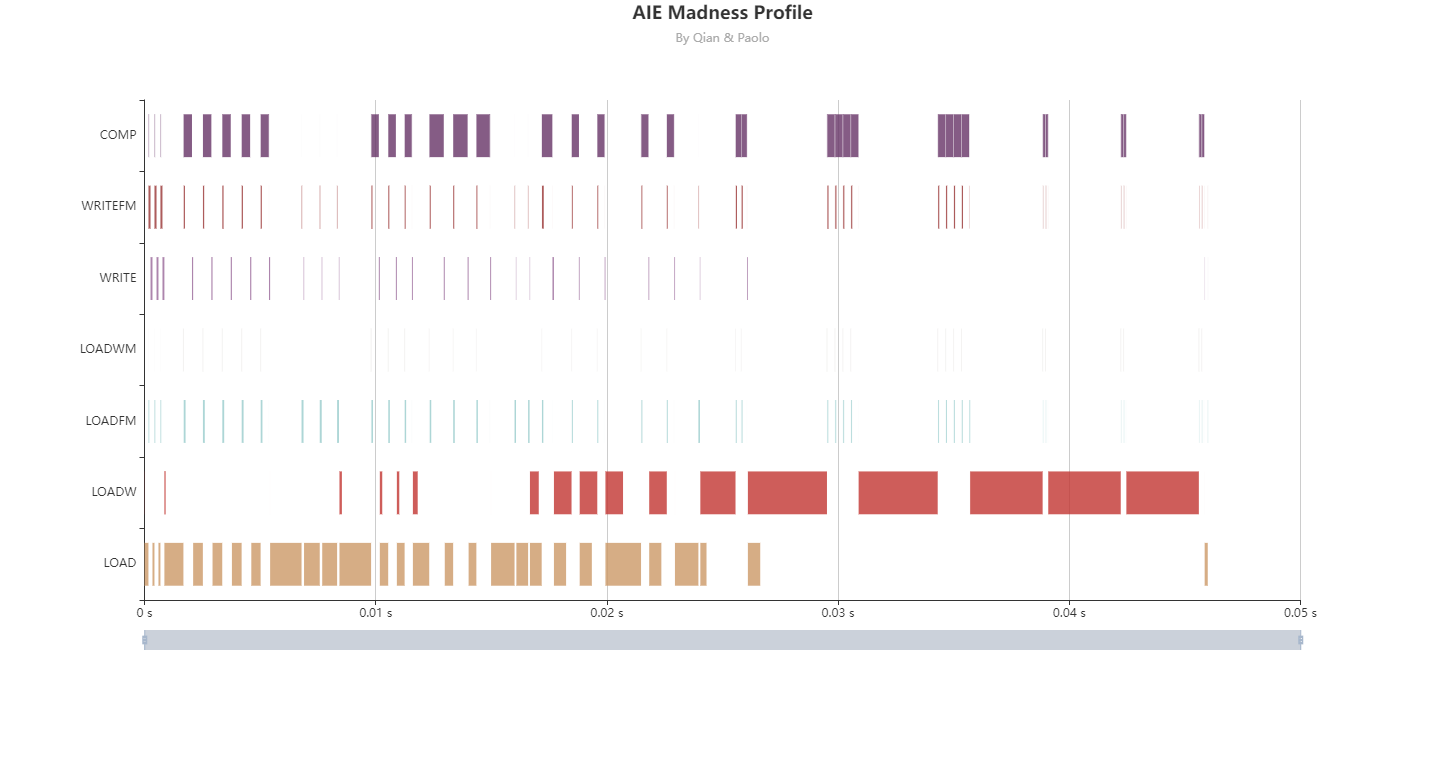
\includegraphics[width=0.99\linewidth]{vgg16overall.png}
\label{vgg16overall}
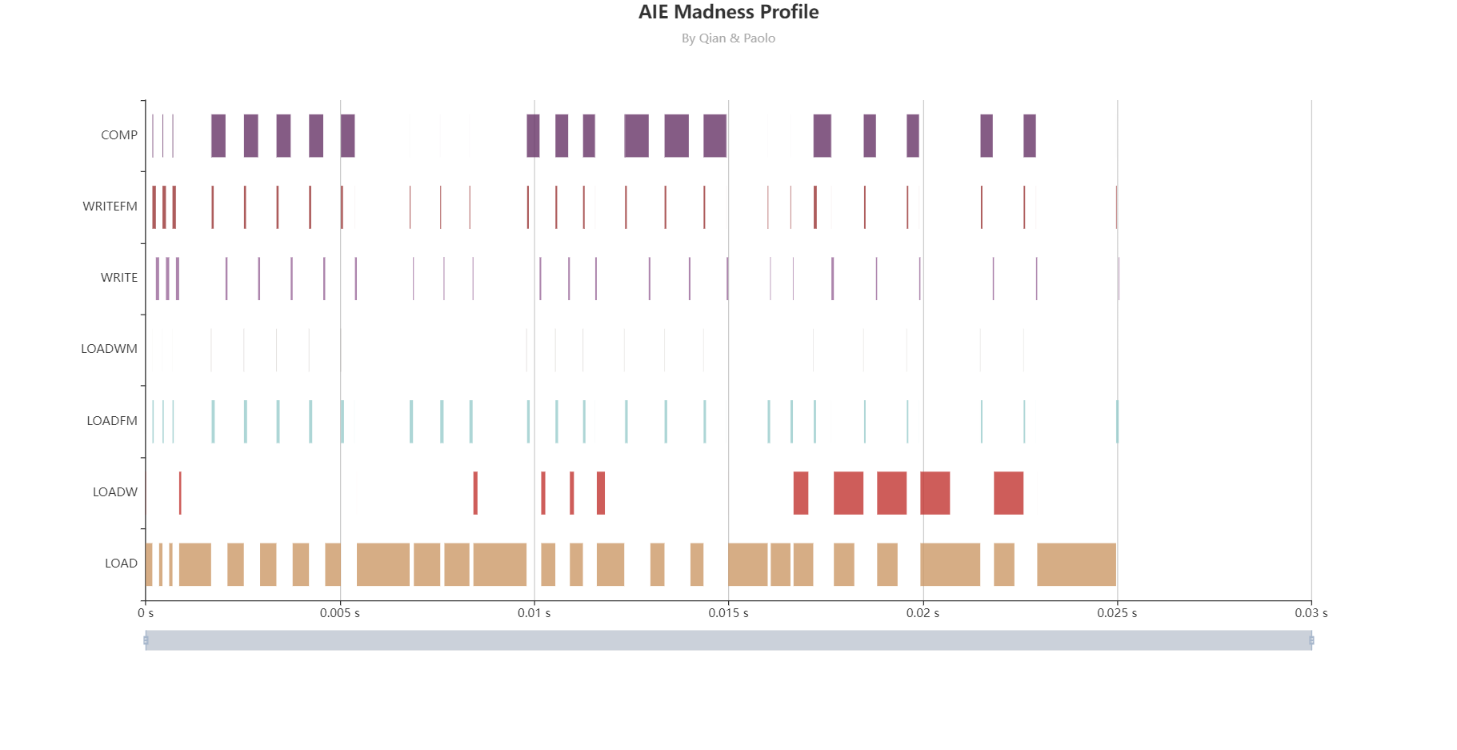
\includegraphics[width=0.99\linewidth]{vggddronly.png}
\caption{VGG16 3x3 DDR only}
\label{vggddronly}
\end{figure}
%\newpage
We apply depth-wise tiling using three tiles 0.024s and we break
even. With two tiles, we achieve better performance at 0.022s, see
Figure \ref{vgg3tiles} and \ref{vgg2tiles}. Sparsity by itself without
any tiling can achieve only 0.021s. Sparsity and tiling improves even
further and we achieve 0.014s, see Figure \ref{vgg2tilessparse}. A
posteriori, we can appreciate the reduction of activation DDR
communications thanks to depth-wise tiling and the reduction of
computation and weights communication by sparsity. 
\begin{figure}[htb]
\centering 
\caption{VGG16 3x3 DDR only 3 tiles}
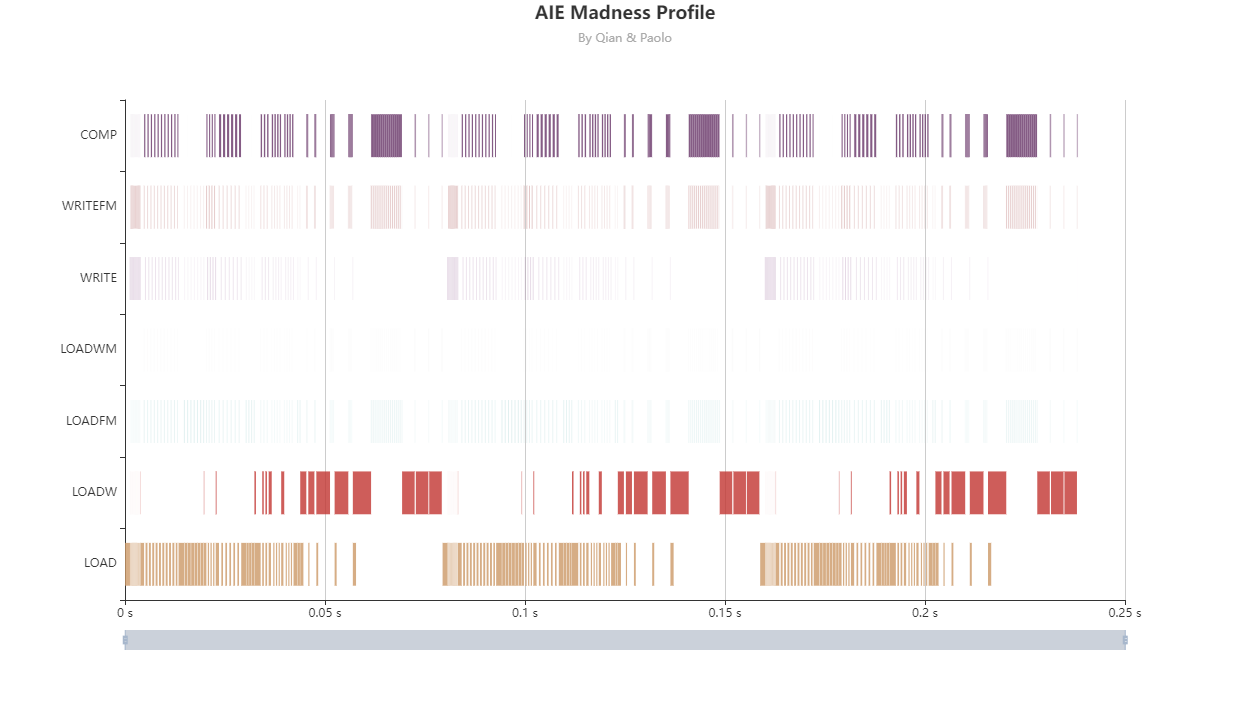
\includegraphics[width=0.99\linewidth]{vgg3tiles.png}
\label{vgg3tiles}
\caption{VGG16 3x3 DDR only 2 tiles}
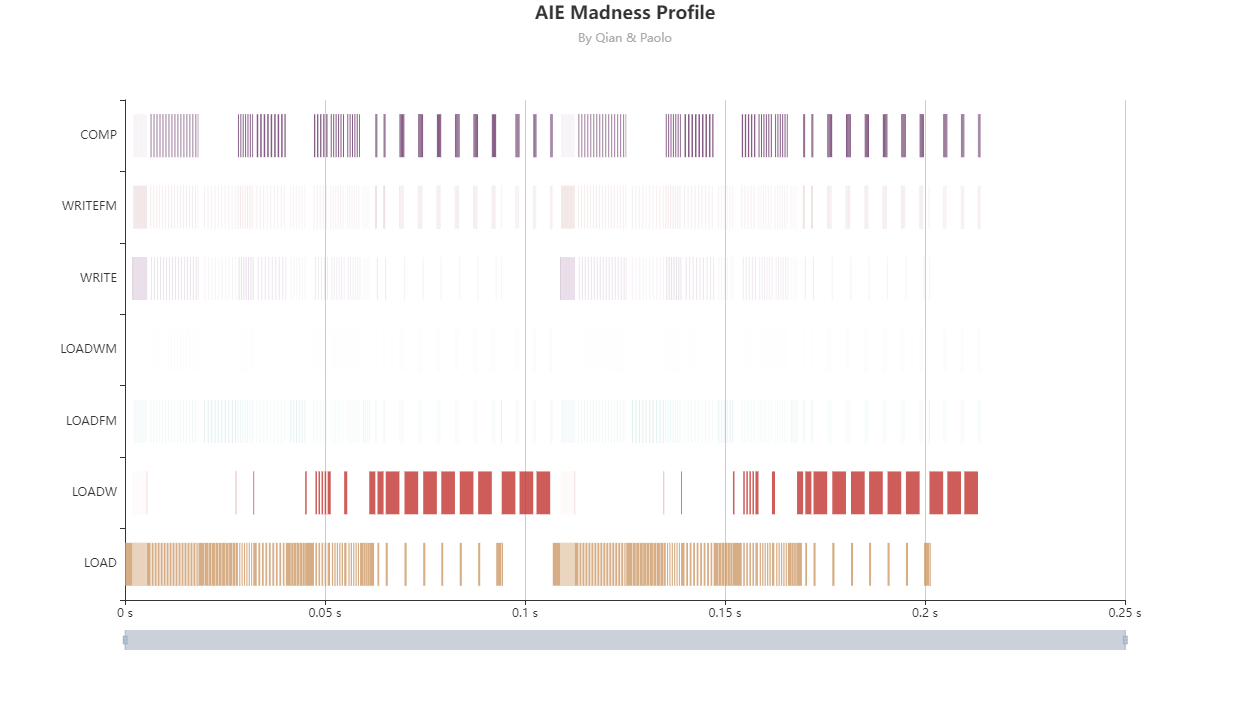
\includegraphics[width=0.99\linewidth]{vgg2tiles.png}
\label{vgg2tiles}
\caption{VGG16 3x3 DDR only 2 tiles sparse}
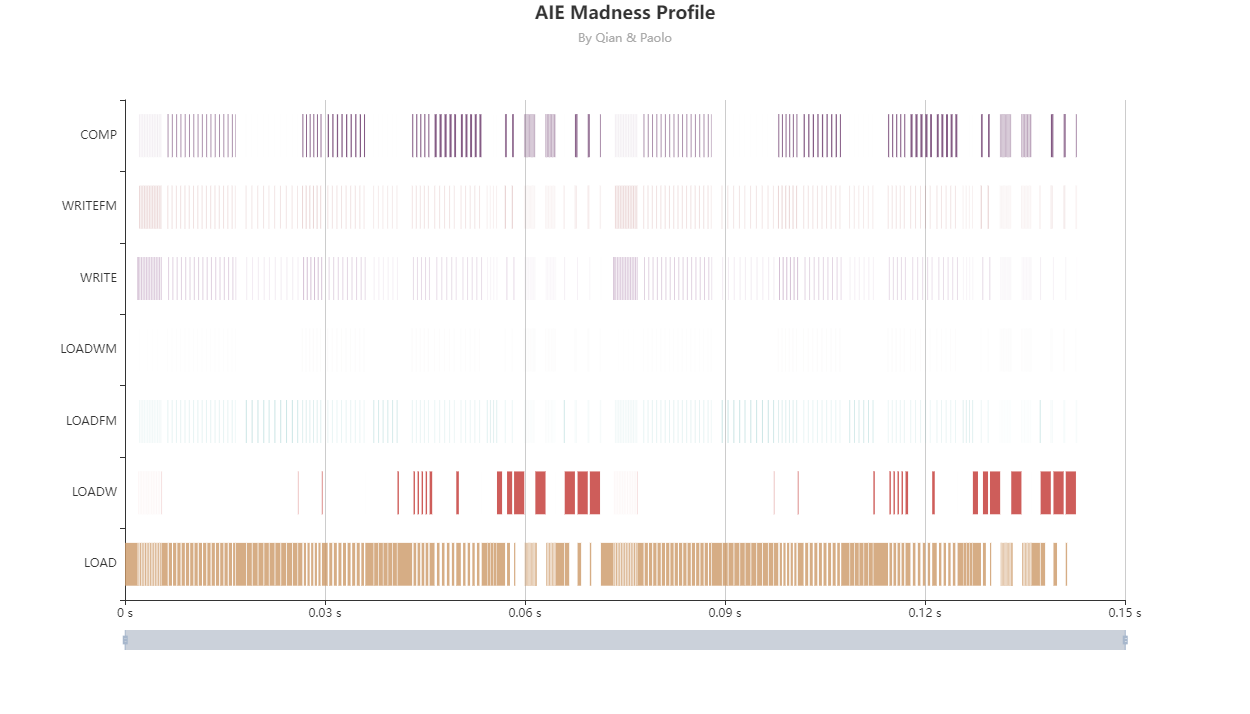
\includegraphics[width=0.99\linewidth]{vgg2tilessparse.png}
\label{vgg2tilessparse}
\end{figure}





\section{Conclusions and Context}
This is a multifaceted problem and we present a complete solution from
training techniques, compilers, code generation, HW definition, and
time estimations.

This could be seen as a quantization and sparsification problem on how
to reduce the footprint of a CNN network. There are post-training
techniques that are targeting quantization and unstructured sparsity
\cite{frantar2023gptq} and all the reference within and its
citations. For the type of sparsity we are planning, we need to be
more aggressive and trai for it (as starting point
\cite{abs-2102-11289}).  But our sparsity is not really a property of
the model, it is a sparsity that the software can describe and the
hardware can take advantage without having any hardware support.

This work stemmed from a collaboration between Xilinx and Numenta and
the idea set forward by the authors in \cite{ahmad2019dense}, where
the models are too dense and there is a lot of room for
improvements. Sparsity at the beginning was proposed for weights with
blocks $4\times 4$ and for activations (a ReLU zeros a lot and there
have been prototypes programming logic was added to AIE1 fabric to
support top-k run-time activations). We must thanks Vamsi Nalluri for
the AIE1 prototype and the original contribution to the AIE2. With the
new AIE2 and logic, the run-time support and top-k was dropped. The
compiler could and can do average estimate of tensor contents but we
do not have run-time support for dynamic and unstructured
sparsity. New support is coming like the 2 over 4 (4 over 8) sparsity
but it is not clear how it will affect the activation encoding and
total accuracy. In principle, we could use 2 by 4 zero encoding for
the non-zero blocks to further reduce space and computations.

This is the second attempt to create time estimates given a specific
AIE configurations. Sourabh Donfaonkar designed the first estimate
model to shape the architecture and optimize the code for $8\times 2$
cohort row by column with two memtiles per column, within a $8\times
8$ shim (i.e., block), and composition of 9-10 of them. This first
step investigates how split the weight by CIN and by COUT and how the
random block sparsity affects the coding and actual memory foot-print
(HW loves symmetric computations and unbalance computations will
be reduce to balanced ones). This shaped our understanding how to
compress weights. Now, we write instructions with the intent of
executing them, we know where the data will be and what amount we
shall move, and thus we account for most of the idiosyncrasies of the
model (padding and strides) and of the communications (yes, padding).


The difficulty of generating code for complex architectures can be
described and solved in different ways. There are recent attempts of
introducing SW/HW solution for spatial processors like ours
\cite{Huang2021CoSASB,Russo2023MemoryAwareDA,Cai2023InterlayerSS}. The
main difference:
\begin{itemize}
   \item We use software developed for FPGA custom IPs because we can
     reuse the two-level of memory hierarchy abstraction.
   \item We use heuristics to explore scheduling.
   \item We use heuristics to memory allocation.
     \begin{itemize}
     \item There is a memory allocation so temporal locality is
       exploited and different (layer) schedules can be investigated.
     \item All passes know all tensor shapes at compile time (no
       run-time support).
     \end{itemize}
   \item We write {\em all} the data movements and the code can and is
     used by a AIE2 compiler (binary compiler if you like) to create
     executable codes.
     \begin{itemize}
     \item Code generated for $1\times 1$ have been simulated, run and
       validated in HW.
     \item We assume that core to core communication by columns
       (larger kernel and stride require overlapping column data) or
       communication by row (reduction of partial sums) are inherently
       taken care by the kernel computation (in practice they are
       not).
     \item Kernel computation (the basic computation in the AIE2) has
       effects on the shapes and layout of the operands. The HW
       architects instruct the compiler about the tensor requirements.
     \item The compiler does not generate fully correct addresses but
       all the tensor shapes are valid and correct for most $K\times
       K$ of reasonable size $K\leq 8$.
     \end{itemize}
   \item No full or partial simulation is needed, and now time
     estimates can be used to quantify scheduling and HW
     configurations choices. Yes, there is further arbitrary
     connections and hardware configurations that can change and the
     effects are visible only by writing code for it \dots
\end{itemize}

For simplicity, we do not provide all the details about the
compiler and the AIE2 interconnections. This is a working
but-in-progress software system and we intend to make it available in
its entirety as much as we made public some of it.
     
     
\section{appendix}
\label{sec:appendix}



Here, we
present the collection of execution times as images:
\begin{itemize}
  \item Figure \ref{fig:incv3-1} Inception V3 2x2 dense and sparse
  \item Figure \ref{fig:incv3-2} Inception V3 3x3 dense and sparse
  \item Figure \ref{fig:incv3-3} Inception V3 4x4 dense and sparse
  \item Figure \ref{fig:incv3-4} Inception V3 5x5 dense and sparse FAILs
  \item Figure \ref{fig:incv3-5} Inception V3 6x6 dense and sparse 
  \item Figure \ref{fig:incv3-6} Inception V3 8x8 dense and sparse
  \item Figure \ref{fig:incv3-7} Resnet 50 2x2 dense and sparse   
  \item Figure \ref{fig:incv3-8} Resnet 50 3x3 dense and sparse   
  \item Figure \ref{fig:incv3-9} Resnet 50 4x4 dense and sparse   
  \item Figure \ref{fig:incv3-10} Resnet 50 5x5 dense FAILs and sparse   
  \item Figure \ref{fig:incv3-11} Resnet 50 6x6 dense and sparse   
  \item Figure \ref{fig:incv3-12} VGG16  2x2 dense and sparse   
  \item Figure \ref{fig:incv3-13} VGG16  4x4 dense and sparse   
  \item Figure \ref{fig:incv3-14} VGG16  8x8 dense and sparse   
\end{itemize}
\newpage 
\DDoublefigure{1.3}{IncV3-2x2-2share-dense.png}{IncV3-2x2-2share-sparse.png}{Inception
  for 2x2 AIE with dense (left/top) weights and sparse (right/bottom)
}{fig:incv3-1}
\DDoublefigure{1.3}{IncV3-3x3-3share-dense.png}{IncV3-3x3-3share-sparse.png}{Inception
  for 3x3 AIE with dense (left/top) weights and sparse (right/bottom)
}{fig:incv3-2}
\DDoublefigure{1.3}{IncV3-4x4-4share-dense.png}{IncV3-4x4-4share-sparse.png}{Inception
  for 4x4 AIE with dense (left/top) weights and sparse (right/bottom)
}{fig:incv3-3}
\SSinglefigure{2.6}{IncV3-5x5-5share-dense.png}{Inception for 5x5 AIE
  with dense weights and FAILED for sparse weights }{fig:incv3-4}
\DDoublefigure{1.3}{IncV3-6x6-6share-dense.png}{IncV3-6x6-6share-sparse.png}{Inception
  for 6x6 AIE with dense (left/top) weights and sparse (right/bottom)
}{fig:incv3-5}
\DDoublefigure{1.3}{IncV3-8x8-8share-dense.png}{IncV3-8x8-8share-sparse.png}{Inception
  for 8x8 AIE with dense (left/top) weights and sparse (right/bottom)
}{fig:incv3-6}
\DDoublefigure{1.3}{Res2x2-2share-dense.png}{Res2x2-2share-sparse.png}{Resnet
  for 2x2 AIE with dense (left/top) weights and sparse (right/bottom)
}{fig:incv3-7}
\DDoublefigure{1.3}{Res3x3-3share-dense.png}{Res3x3-3share-sparse.png}{Resnet
  for 3x3 AIE with dense (left/top) weights and sparse (right/bottom)
}{fig:incv3-8}
\DDoublefigure{1.3}{Res4x4-4share-dense.png}{Res4x4-4share-sparse.png}{Resnet
  for 4x4 AIE with dense (left/top) weights and sparse (right/bottom)
}{fig:incv3-9}
\SSinglefigure{2.6}{Res5x5-5share-sparse.png}{Resnet for 5x5 AIE with
  sparse weights and FAILED for dense weights}{fig:incv3-10}
\DDoublefigure{1.3}{Res6x6-6share-dense.png}{Res6x6-6share-sparse.png}{Resnet
  for 6x6 AIE with dense (left/top) weights and sparse (right/bottom)
}{fig:incv3-11}

\DDoublefigure{0.9}{VGG162x2-2shared-dense.png}{VGG162x2-2shared-sparse.png}{VGG 16 (No FC)  for 2x2 AIE with dense (left/top) weights and sparse (right/bottom)}{fig:incv3-12}
\DDoublefigure{0.9}{VGG164x4-4shared-dense.png}{VGG164x4-4shared-sparse.png}{VGG 16 (No FC)  for 4x4 AIE with dense (left/top) weights and sparse (right/bottom)}{fig:incv3-13}
\DDoublefigure{0.9}{VGG168x8-8shared-dense.png}{VGG168x8-8shared-sparse.png}{VGG 16 (No FC)  for 8x8 AIE with dense (left/top) weights and sparse (right/bottom)}{fig:incv3-14}




%%%%%%%%% -- BIB STYLE AND FILE -- %%%%%%%%
\bibliographystyle{IEEEtran} \bibliography{ref}
%%%%%%%%%%%%%%%%%%%%%%%%%%%%%%%%%%%%

%\appendix{Review and Response}
%\input{review.tex}
\end{document}
